\documentclass[11pt]{article}
\setlength\parindent{10pt}
\usepackage{booktabs, natbib, amsmath, amssymb, mathrsfs, tabularx, booktabs, makecell}
\usepackage[margin=1in]{geometry}
\usepackage{caption}
\usepackage{authblk}
\usepackage{graphicx}
\usepackage{csquotes}
\usepackage{hyperref}
\pagestyle{plain}

\captionsetup[table]{skip=10pt}
\captionsetup[figure]{skip=10pt}

\title{Spectral Influence of Researchers:\\
An Open Alternative to the Standardized Citation Metrics Author Database}

\author[1]{Domingo Docampo}
\author[2]{Lawrence Cram}

\affil[1]{Atlantic Research Center for Information and Communication Technologies \newline
University of Vigo, Vigo, Spain}
\affil[2]{Research School of Physics, Australian National University, Canberra, 2600, ACT, Australia \newline
Charles Darwin University, Brinkin, 0810, NT, Australia}

\date{\today}

% numbers generated by researchers/compare_stanford.py
% generated by researchers/compare_stanford.py — do not edit
\newcommand{\NOaAuthors}{28{,}652{,}429}  % oa authors
\newcommand{\NOaEligible}{8{,}240{,}231}  % oa eligible
\newcommand{\NStPopul}{23{,}239{,}426}  % st popul
\newcommand{\NStCareer}{243{,}949}  % st career
\newcommand{\NStSingle}{249{,}310}  % st single
\newcommand{\NRankedPubvFull}{7{,}439{,}124}  % ranked pubv_full
\newcommand{\NRankedPubvFrac}{7{,}439{,}124}  % ranked pubv_frac
\newcommand{\NRankedCvFullAll}{6{,}987{,}387}  % ranked cv_full_all
\newcommand{\NRankedCvFracAll}{6{,}987{,}387}  % ranked cv_frac_all
\newcommand{\NRankedCvFullNs}{6{,}745{,}298}  % ranked cv_full_ns
\newcommand{\NRankedCvFracNs}{6{,}745{,}298}  % ranked cv_frac_ns
\newcommand{\NRankedCvFullSingleall}{5{,}117{,}747}  % ranked cv_full_25all
\newcommand{\NRankedCvFracSingleall}{5{,}117{,}747}  % ranked cv_frac_25all
\newcommand{\NRankedCvFullSinglens}{4{,}889{,}912}  % ranked cv_full_25ns
\newcommand{\NRankedCvFracSinglens}{4{,}889{,}912}  % ranked cv_frac_25ns
\newcommand{\NStPersons}{347{,}131}  % st persons
\newcommand{\NMatchMatched}{261{,}926}  % match matched
\newcommand{\NMatchAmbiguous}{1{,}821}  % match ambiguous
\newcommand{\NMatchImplausible}{10{,}782}  % match implausible
\newcommand{\NMatchConflict}{1{,}697}  % match conflict
\newcommand{\NMatchUnmatched}{70{,}905}  % match unmatched
\newcommand{\NMatchCareerPct}{81.0}  % match career pct
\newcommand{\NMatchSinglePct}{74.8}  % match single pct
\newcommand{\NMatchedCareer}{197{,}566}  % matched career
\newcommand{\NMatchedSingle}{186{,}573}  % matched single
\newcommand{\NCheckNcRho}{0.84}  % check nc rho
\newcommand{\NCheckHRho}{0.94}  % check h rho
\newcommand{\NRhoPubfracC}{0.32}  % rho pubfrac c
\newcommand{\NRhoCitfracnsCns}{0.27}  % rho citfracns cns
\newcommand{\NRhoCitfullallC}{0.28}  % rho citfullall c
\newcommand{\NFieldRhoMin}{0.13}  % field rho min
\newcommand{\NFieldRhoMax}{0.42}  % field rho max
\newcommand{\NFieldMin}{Physics \& Astronomy}  % field min
\newcommand{\NFieldMax}{Public Health \& Health Services}  % field max
\newcommand{\NRhoCitfracnsNcpp}{0.38}  % rho citfracns ncpp
\newcommand{\NRhoPubfracNcpp}{0.50}  % rho pubfrac ncpp
\newcommand{\NTopNCitfracns}{134{,}780}  % top n citfracns
\newcommand{\NTopInStCitfracns}{3.1}  % top in st citfracns
\newcommand{\NStInTopCitfracns}{2.1}  % st in top citfracns
\newcommand{\NTopInStPubfrac}{9.2}  % top in st pubfrac
\newcommand{\NTopMedWorksCit}{10}  % top med works cit
\newcommand{\NTopMedWorksPub}{12}  % top med works pub
\newcommand{\NStMedWorks}{101}  % st med works
\newcommand{\NMedPubAll}{1.08}  % med pub all
\newcommand{\NMedPubSt}{1.51}  % med pub st
\newcommand{\NSharePubAboveOneSt}{88.1}  % share pub above one st
\newcommand{\NSharePubAboveOneAll}{56.4}  % share pub above one all
\newcommand{\NMedCitAll}{1.26}  % med cit all
\newcommand{\NMedCitSt}{1.48}  % med cit st
\newcommand{\NShareCitAboveOneSt}{94.0}  % share cit above one st
\newcommand{\NShareCitAboveOneAll}{76.0}  % share cit above one all
\newcommand{\NAllMedWorks}{12}  % all med works
\newcommand{\NTopMedCitesCit}{196}  % top med cites cit
\newcommand{\NStMedCites}{3{,}346}  % st med cites
\newcommand{\NStInTopPubfrac}{6.9}  % st in top pubfrac
\newcommand{\NShareUsSt}{37.3}  % share US st
\newcommand{\NShareUsCit}{41.6}  % share US cit
\newcommand{\NShareUsPub}{58.4}  % share US pub
\newcommand{\NShareUsAll}{17.1}  % share US all
\newcommand{\NShareCnSt}{6.0}  % share CN st
\newcommand{\NShareCnCit}{8.9}  % share CN cit
\newcommand{\NShareCnPub}{5.0}  % share CN pub
\newcommand{\NShareCnAll}{18.1}  % share CN all
\newcommand{\NShareAuSt}{3.5}  % share AU st
\newcommand{\NShareAuCit}{2.0}  % share AU cit
\newcommand{\NShareAuPub}{1.4}  % share AU pub
\newcommand{\NShareAuAll}{1.8}  % share AU all
\newcommand{\NShareGbSt}{8.8}  % share GB st
\newcommand{\NShareGbCit}{6.8}  % share GB cit
\newcommand{\NShareGbPub}{9.0}  % share GB pub
\newcommand{\NShareGbAll}{3.6}  % share GB all
\newcommand{\NShareInSt}{1.6}  % share IN st
\newcommand{\NShareInCit}{0.8}  % share IN cit
\newcommand{\NShareInPub}{0.4}  % share IN pub
\newcommand{\NShareInAll}{4.0}  % share IN all
\newcommand{\NSelfRho}{0.85}  % self rho
\newcommand{\NSelfMedOurs}{12.1}  % self med ours
\newcommand{\NSelfMedSt}{11.8}  % self med st
\newcommand{\NSelfMedAll}{13.0}  % self med all
\newcommand{\NSelfOverForty}{250{,}992}  % self over forty
\newcommand{\NSelfBase}{6{,}195{,}414}  % self base
\newcommand{\NSelfOverFortyPct}{4.1}  % self over forty pct
\newcommand{\NStSelfOverFortyPct}{1.1}  % st self over forty pct
\newcommand{\NRhoCitAllNs}{0.97}  % rho cit all ns
\newcommand{\NSelfShiftMed}{2.1}  % self shift med
\newcommand{\NSelfShiftNinety}{10.3}  % self shift ninety
\newcommand{\NSelfHiShift}{-1.2}  % self hi shift
\newcommand{\NSelfHiGain}{1.2}  % self hi gain
\newcommand{\NRhoPubFullFrac}{0.99}  % rho pub full frac
\newcommand{\NRhoCitFullFrac}{0.98}  % rho cit full frac
\newcommand{\NRhoCitCareerSingle}{0.79}  % rho cit career single
\newcommand{\NAuEligible}{125{,}303}  % au eligible
\newcommand{\NAuStCareer}{8{,}551}  % au st career
\newcommand{\NAuTopCitfracns}{2{,}294}  % au top citfracns
\newcommand{\NAuTopPubfrac}{1{,}744}  % au top pubfrac


\begin{document}
\maketitle

\begin{abstract}
The standardized citation metrics author database of Ioannidis and colleagues, widely known as the Stanford top-2\% list, ranks researchers by a composite of six cumulative citation indicators computed from Scopus. We describe an open alternative built from OpenAlex and from the bipartite spectral ranking of sources and institutions. Each work receives a publication score, from the size-independent influence of its source and institutions, and a citer score, the mean influence of the sources of the works that cite it. A researcher's score is the mean over their papers, with full or fractional counting and with or without self-citations. We compute scores for the \NOaEligible{} OpenAlex authors who meet the Stanford volume baseline of five papers and match \NMatchCareerPct{}\% of the Stanford career table to OpenAlex authors by name, location and volume. Self-citation shares measured in the two databases agree closely (Spearman \NSelfRho{}). Spectral scores correlate weakly with the Stanford composite among listed researchers (0.27--0.32) and more strongly with Stanford citations per paper (up to \NRhoPubfracNcpp{}), and top-2\% lists drawn up on spectral scores overlap little with the Stanford list, because a mean rewards the typical reception of a researcher's papers rather than their total. Removing self-citations barely changes the citer score and raises it for heavy self-citers, whose self-citations come from less influential sources. An influence-weighted mean therefore offers an author-level indicator that is open, field-normalised and difficult to inflate by self-citation, at the cost of favouring short records unless combined with a measure of volume.

\end{abstract}

% !TeX root = ../main.tex
% ---------------------------------------------------------------
\section{Introduction}
\label{sec:introduction}
% ---------------------------------------------------------------

Lists of highly cited researchers carry weight well beyond bibliometrics. Universities cite them in promotion cases and press releases, ranking agencies use them as inputs, and funders and governments read them as signals of national standing. Since 2019 the most widely used of these lists has been the standardized citation metrics author database produced by Ioannidis and colleagues from Scopus, commonly known as the Stanford ``top 2\%'' list \citep{ioannidisStandardizedCitationMetrics2019a, ioannidisUpdatedSciencewideAuthor2020}. The database reports, for every author with at least five papers, six citation indicators and a composite $c$ that combines them \citep{ioannidisMultipleCitationIndicators2016}. Authors are listed if they are among the 100,000 highest by $c$ or in the top 2\% of their Science-Metrix subfield, with and without self-citations, for career-long citations and for citations received in a single recent year. The ninth version, released in 2026, lists about a quarter of a million researchers in each table.

The Stanford database answers several criticisms of earlier lists. It covers every field to a useful depth, separates self-citations, discounts co-authorship through the $h_m$ index \citep{schreiberCaseStudyArbitrariness2013}, and gives weight to single, first and last authorship. Its authors are explicit that it is not a measure of quality and that inclusion and exclusion should not be over-read. Three features nevertheless limit what it can show. First, $c$ is cumulative. Each of its six components grows with the number of papers and with career length, so the list favours prolific and senior researchers, and the single-year table only partly corrects this \citep{ioannidisStandardizedCitationMetrics2019a}. Second, every citation counts the same, whether it comes from a paper in a leading journal or from one in a venue that is rarely read, so the indicators are open to citation cartels and other forms of manipulation that the database's authors themselves have documented \citep{ioannidisGeneralizedViewSelfcitation2015, szomszorHowMuchToo2020}. Third, the database is built from a proprietary source, and its author profiles, field assignments and citation links cannot be inspected or reproduced outside Elsevier.

This paper describes an alternative built on open data and on a different idea of what an author-level indicator should measure. We start from the bipartite spectral ranking of sources and institutions of \citet{docampodomingoRecirculatingCardinalSpectral2026}, computed from OpenAlex \citep{priemOpenAlexFullyopenIndex2022}, which assigns every journal and institution in a field a size-independent influence $v$ with field mean one. Each work then inherits two scores: a publication score, from the influence of the source and institutions that produced it, and a citer score, the mean influence of the sources of the works that cite it. A researcher's score is the mean of these work scores over their papers, under full or fractional counting and with or without self-citations. The resulting indicators measure the typical standing of a researcher's papers rather than their volume, and they weight citations by where they come from.

We ask three questions. How many researchers can be scored at the volume threshold that the Stanford database uses, and how many of the Stanford-listed researchers can be found in OpenAlex? How closely do spectral scores agree with the Stanford indicators, and where they disagree, is the disagreement associated with field, country, self-citation or co-authorship? And how different would a top-2\% list be if it were drawn up on spectral scores rather than on $c$?

The paper proceeds as follows. Section~\ref{sec:spectral_ranking} sets out the spectral ranking and the work and researcher scores derived from it. Section~\ref{sec:data} describes the OpenAlex corpus, the volume threshold, the Stanford database and the matching of Stanford authors to OpenAlex. Section~\ref{sec:results} reports coverage, agreement and the composition of the two lists, and Section~\ref{sec:discussion} discusses what the comparison shows and what it does not.

% !TeX root = ../main.tex
% ---------------------------------------------------------------
\section{From Sources and Institutions to Researchers}
\label{sec:spectral_ranking}
% ---------------------------------------------------------------

\subsection{Spectral influence of sources and institutions}

We use the bipartite spectral ranking of \citet{docampodomingoRecirculatingCardinalSpectral2026}, computed separately for each of the 26 OpenAlex fields $F$. Sources and institutions enter a field by publishing a minimum volume of field-weighted works in the ranking window, where a work's weight $f_{wF}$ in field $F$ is the sum of its subfield weights in that field. References among the retained works link sources to institutions and institutions to sources. Each reference is weighted by the mean field weight of the two works and by the inverse length of the referencing work's filtered reference list, and an institution's share of a work is fractionated over authors and their affiliations \citep{waltmanFieldnormalizedCitationImpact2015}. Row-normalising the resulting source--institution reference matrix gives a bipartite transition matrix $\mathbf{H}$. Its square separates into one-mode operators for sources and for institutions \citep{breigerDualityPersonsGroups1974}, and the Perron vector of the source operator gives the stationary ranking probability $\pi_p$ of every unit $p$. The size-independent influence is
\begin{equation}
  v_p = \frac{A}{a_p}\,\pi_p ,
  \label{eq:v}
\end{equation}
where $a_p$ is the field-weighted work count of unit $p$ and $A = \sum_p a_p$, so that the output-weighted mean of $v$ over the units of a field is one \citep{pinskiCitationInfluenceJournal1976, palacios-huertaMeasurementIntellectualInfluence2004}. A source or institution with $v = 2$ attracts twice the field-average influence per unit of output. The model, its parameters and its convergence diagnostics are set out in \citet{docampodomingoRecirculatingCardinalSpectral2026}. Here we use the baseline settings of that paper, with the ranking window 2020--2024.

\subsection{Spectral scores of works}

The ranking scores sources and institutions, not works or people. We attach two scores to each work, both derived from the influence of the units involved.

The \emph{publication score} describes where, and from which institutions, a work was published. In field $F$ the work score is the mean of the influence of its source and the unweighted mean influence of its retained institutions, $u_{wF} = \frac{1}{2}\big(v_{S(w)} + \bar{v}_{I(w)}\big)$, falling back to $v_{S(w)}$ when none of the work's institutions is retained. A work that appears in several fields has the field-weighted mean
\begin{equation}
  u_w = \frac{\sum_F f_{wF}\, u_{wF}}{\sum_F f_{wF}} ,
  \label{eq:pubv}
\end{equation}
taken over the fields in which its source is retained. The publication score is fixed when a work appears. It does not depend on who later cites the work, so self-citation cannot alter it.

The \emph{citer score} describes who cites a work. Each citing work $c$ is assigned the influence of its source, taking the largest value over the fields in which that source is retained, $v_c = \max_F v_{S(c),F}$; this is the convention we used for highly cited works in an earlier study of citation enclaves. For a work $w$ with a set $\mathcal{C}_w$ of citing works that carry a score, the citer score is
\begin{equation}
  \langle v \rangle_w = \frac{1}{|\mathcal{C}_w|} \sum_{c \in \mathcal{C}_w} v_c .
  \label{eq:citerv}
\end{equation}
It is a mean, not a sum, so a work cited by a few papers in highly influential sources scores higher than a work cited by many papers in sources of average influence. Citing works whose source is not retained in any field carry no score and are omitted. We compute $\langle v \rangle_w$ in two versions. In the first, $\mathcal{C}_w$ contains every citing work. In the second, it excludes self-citations, defined as in the Stanford database: a citing work is a self-citation of $w$ when it shares at least one author with $w$ \citep{ioannidisStandardizedCitationMetrics2019a}. We also compute single-year versions, in which $\mathcal{C}_w$ is restricted to citing works published in 2025, the year of the Stanford single-year table.

\subsection{Spectral scores of researchers}

A researcher's score is the mean of the work scores over that researcher's works. Let $W_a$ be the works of author $a$ that are articles, reviews or conference papers, and let $n_w$ be the number of authors of work $w$. Under full counting each work has weight $\phi_w = 1$; under fractional counting it has weight $\phi_w = 1/n_w$, so that a single-authored paper counts as much as twenty papers with twenty authors each. The two researcher scores are the weighted means
\begin{equation}
  V^{\mathrm{pub}}_a = \frac{\sum_{w \in W_a} \phi_w\, u_w}{\sum_{w \in W_a} \phi_w} , \qquad
  V^{\mathrm{cit}}_a = \frac{\sum_{w \in W_a^{c}} \phi_w\, \langle v \rangle_w}{\sum_{w \in W_a^{c}} \phi_w} ,
  \label{eq:author_v}
\end{equation}
where the first sum runs over the works that have a publication score and the second over the subset $W_a^{c}$ that has at least one scored citing work. Uncited works are left out of $V^{\mathrm{cit}}$, and the number of cited works is reported alongside it. With two counting rules, citations with and without self-citations, and career and single-year citation windows, there are two publication scores and eight citer scores per researcher.

Both scores are size-independent in the same sense as $v$. They describe the typical standing of a researcher's work, not its total volume or its total citations. A researcher with many papers is not ranked above one with few unless the papers score higher on average. This is the main conceptual difference from the composite indicator $c$ of the Stanford database, which combines six cumulative citation counts and indices and therefore rises with productivity \citep{ioannidisMultipleCitationIndicators2016}. The scores are also field-normalised by construction, because $v$ has mean one within every field, whereas the Stanford database leaves normalisation to the user through subfield percentiles.

% !TeX root = ../main.tex
% ---------------------------------------------------------------
\section{Data}
\label{sec:data}
% ---------------------------------------------------------------

\subsection{OpenAlex corpus and eligible researchers}

The corpus is drawn from the October 2026 snapshot of OpenAlex \citep{priemOpenAlexFullyopenIndex2022}. It contains works published from 2000 to 2025 in journals, conference proceedings and book series, of nine work types, with at most 29 authors, after removal of duplicate titles. The spectral rankings of sources and institutions use the works of 2020--2024 and are computed for each of the 26 OpenAlex fields. Work scores are then attached to every corpus work whose source is retained in at least one field, whatever its publication year, so a paper of 2005 is scored by the present-day influence of its journal and institutions and by the influence of the sources that cite it.

Authors are identified by the OpenAlex author identifier. Following the volume baseline of the Stanford database, which reports percentiles for every author with at least five papers \citep{ioannidisStandardizedCitationMetrics2019a}, we treat as eligible every author with at least five corpus works of type article, review or conference paper. Of the \NOaAuthors{} authors with at least one corpus work, \NOaEligible{} are eligible. For comparison, the field tables of the Stanford database count \NStPopul{} Scopus authors with at least five papers. The difference probably reflects Scopus's longer time span, its broader coverage of document types and large collaborations, and differences in author disambiguation. Researcher scores are computed over the eligible authors' articles, reviews and conference papers only, and a score is ranked only when it rests on at least five works: five works with a publication score, or five cited works for a citer score.

Two features of OpenAlex author records bear on the results. Author disambiguation is algorithmic and imperfect, so some researchers are split across several identifiers and some identifiers merge different people. And the corpus omits papers with 30 or more authors, which removes the large-collaboration papers of particle physics, astronomy and genomics that weigh heavily in the Stanford indicators for those fields.

\subsection{The Stanford database}

We use version 9 of the database, released in August 2026 and built from a Scopus snapshot of 1 August 2026 \citep{ioannidisUpdatedSciencewideAuthor2020}. The career table lists \NStCareer{} researchers on citations received from 1996 to 2025 to papers published since 1960. The single-year table lists \NStSingle{} researchers on citations received in 2025. Each row gives the researcher's name, one institution and country, the number of papers, the six component indicators and $c$ with and without self-citations, the self-citation share, and the researcher's main Science-Metrix field and subfields. Scopus author identifiers are not included.

\subsection{Matching Stanford researchers to OpenAlex}

Without a shared identifier, Stanford researchers must be matched to OpenAlex authors by name. We pool the two tables into \NStPersons{} distinct persons. Candidates are eligible OpenAlex authors who have a name variant, on any of their authorships, with the same surname and first initial, whose affiliations include the Stanford country, and whose $h$-index is within a factor of 2.5 of the Stanford career $h$. For persons who appear only in the single-year table, whose $h$ counts 2025 citations alone, the paper count is compared instead. The five candidates closest in paper count and $h$ are then scored. The author's canonical OpenAlex name must contain the Stanford surname and must agree on given names: full given names must coincide once concatenated (so that Zhong Lin matches Zhonglin but Yanfei does not match Yan), and initials must agree as far as both names give them. Candidates whose names agree only in initials are accepted only when one of their OpenAlex affiliations matches the Stanford institution. Among the remaining candidates, the score rewards an institutional match, agreement of middle initials and closeness in volume, and a person is matched when the best candidate leads the next by a clear margin. An OpenAlex author claimed by two persons is kept for the stronger claim. On this rule \NMatchMatched{} persons are matched, covering \NMatchCareerPct{}\% of the career table and \NMatchSinglePct{}\% of the single-year table.

The match can be checked against quantities that both databases measure. Across matched career-table researchers, the Spearman correlation between Stanford's total citation count and the number of corpus citations to the researcher's OpenAlex works is \NCheckNcRho{}, and between the Stanford and OpenAlex $h$-indices it is \NCheckHRho{}. Both are well short of one, because Scopus and OpenAlex differ in coverage and the corpus starts in 2000, but they are high enough to indicate that the matched records mostly describe the same people. A random sample of 100 matches was also inspected by hand (Section~\ref{sec:results}).

% !TeX root = ../main.tex
% ---------------------------------------------------------------
\section{Results}
\label{sec:results}
% ---------------------------------------------------------------

\subsection{Coverage and matching}

Of the \NOaEligible{} eligible OpenAlex authors, \NRankedPubvFrac{} have at least five works with a publication score and \NRankedCvFracNs{} have at least five works cited by scored works once self-citations are removed. Restricting citations to those made in 2025 leaves \NRankedCvFracSinglens{} researchers with a single-year citer score. Researchers drop out of a score when fewer than five of their works carry it, which happens when most of their papers appear in sources that are not retained in any field ranking or attract no citations from retained sources.

The matching procedure of Section~\ref{sec:data} assigned an OpenAlex author to \NMatchMatched{} of the \NStPersons{} Stanford persons, covering \NMatchCareerPct{}\% of the career table and \NMatchSinglePct{}\% of the single-year table. The single-year table matches less well. It contains more researchers who began publishing recently (16\% with a first paper in 2012 or later, against 2\% in the career table), whose short records make the volume comparison less discriminating, and its researchers who are not also in the career table have no comparable $h$-index, so their candidates are checked on paper count only. In a hand check of 100 randomly drawn matches, 98 agreed in name, in institution or country, and in paper count and $h$-index. The other two were common English names without an institutional match, which we could neither confirm nor reject. Of the remaining persons, \NMatchUnmatched{} had no candidate that agreed on surname, given name, country and volume, \NMatchImplausible{} had a best candidate identified only by initials and without an institutional match, \NMatchAmbiguous{} had two candidates of similar strength, and \NMatchConflict{} lost their candidate to a stronger claim by another Stanford person.

\subsection{Distribution of researcher scores}

Figure~\ref{fig:distributions} shows the distribution of the fractional scores. The median publication score of eligible researchers is \NMedPubAll{}, and \NSharePubAboveOneAll{}\% of them score above one. Stanford-listed researchers score higher, with a median of \NMedPubSt{} and \NSharePubAboveOneSt{}\% above one. The citer score is centred higher, with medians of \NMedCitAll{} for all eligible researchers and \NMedCitSt{} for Stanford-listed researchers, because the citing works that carry a score are those in retained sources, which on average have higher influence than the sources excluded from the ranking. The citer score is therefore a relative measure. Its value of one does not mark the field average in the way that $v = 1$ does for sources and institutions.

\begin{figure}[t]
\centering
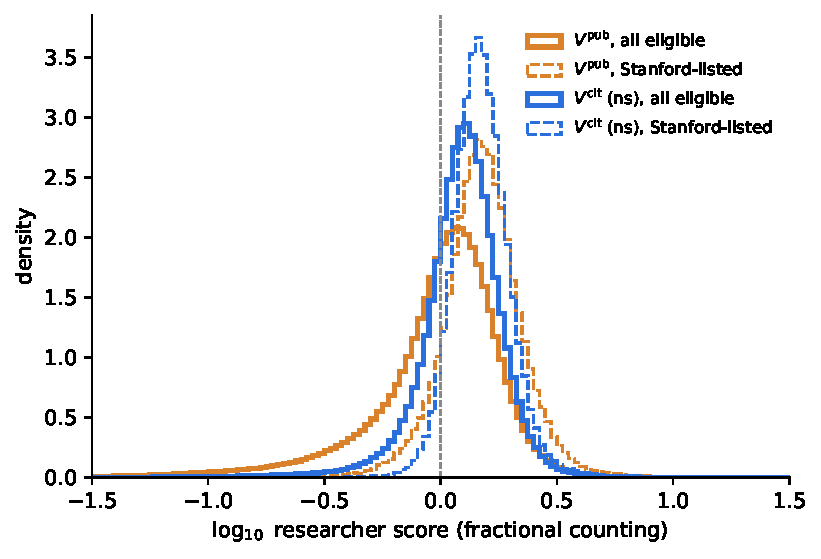
\includegraphics[width=0.7\textwidth]{figures/fig_distributions.pdf}
\caption{Distribution of researcher scores under fractional counting for all eligible OpenAlex researchers (solid) and for researchers matched to the Stanford career table (dashed). Citer scores exclude self-citations. The dashed vertical line marks a score of one.}
\label{fig:distributions}
\end{figure}

\subsection{Agreement with the Stanford indicators}

Among matched researchers, spectral scores and Stanford indicators are only weakly related (Table~\ref{tab:agreement}, Figure~\ref{fig:v_vs_c}). The Spearman correlation between the fractional publication score and $c$ is \NRhoPubfracC{}, and between the fractional citer score without self-citations and $c$ without self-citations it is \NRhoCitfracnsCns{}. Correlations with total citations and with $h$ are lower again, and correlations with the co-authorship-adjusted $h_m$ are close to 0.14 for every score. The single-year scores agree less with the single-year table than the career scores do with the career table.

Two features of the comparison keep these correlations low, and they should not be read as disagreement about the same quantity. The first is range restriction. The matched researchers are all in the top 2\% of their subfield or the top 100,000 by $c$, so the comparison is made within a narrow upper band of the $c$ distribution. The second, and more important, is that $c$ is cumulative and the spectral scores are means. When Stanford's citations are divided by papers to give a size-independent rate, the correlation with the fractional citer score rises to \NRhoCitfracnsNcpp{}, and with the fractional publication score to \NRhoPubfracNcpp{}. Within Stanford fields (Table~\ref{tab:fields}), the correlation of the citer score with $c$ ranges from \NFieldRhoMin{} in \NFieldMin{} to \NFieldRhoMax{} in \NFieldMax{}. The low value in physics is probably related to the exclusion of papers with 30 or more authors from the OpenAlex corpus, which removes much of the citation record on which $c$ rests in parts of that field.

\begin{table}[t]
\centering
\caption{Spearman correlations between spectral researcher scores and Stanford indicators for matched researchers with at least five contributing works. Career scores are compared with the career table and single-year (2025) citer scores with the single-year table. ``pub'' is the publication score, ``cit'' the citer score, ``ns'' excludes self-citations, and ``full'' and ``frac'' denote full and fractional counting. Stanford indicators include self-citations except for $c$ (ns).}
\label{tab:agreement}
\small
% generated by researchers/compare_stanford.py
\begin{tabular}{lrrrrrr}
\toprule
Spectral score & $c$ & $c$ (ns) & $n_c$ & $h$ & $h_m$ & $N$ \\
\midrule
pub, full & 0.32 & 0.36 & 0.33 & 0.25 & 0.13 & 196{,}223 \\
pub, frac & 0.32 & 0.37 & 0.32 & 0.25 & 0.14 & 196{,}223 \\
cit, full & 0.28 & 0.30 & 0.23 & 0.17 & 0.14 & 196{,}909 \\
cit, frac & 0.27 & 0.30 & 0.22 & 0.16 & 0.14 & 196{,}909 \\
cit, full, ns & 0.26 & 0.28 & 0.19 & 0.14 & 0.13 & 196{,}791 \\
cit, frac, ns & 0.25 & 0.27 & 0.18 & 0.13 & 0.13 & 196{,}791 \\
\midrule
cit 2025, full $\to$ single-yr & 0.23 & 0.25 & 0.11 & 0.12 & 0.15 & 184{,}419 \\
cit 2025, frac $\to$ single-yr & 0.22 & 0.24 & 0.10 & 0.11 & 0.16 & 184{,}419 \\
cit 2025, full, ns $\to$ single-yr & 0.22 & 0.24 & 0.08 & 0.10 & 0.15 & 184{,}292 \\
cit 2025, frac, ns $\to$ single-yr & 0.22 & 0.23 & 0.07 & 0.09 & 0.16 & 184{,}292 \\
\bottomrule
\end{tabular}

\end{table}

\begin{figure}[t]
\centering
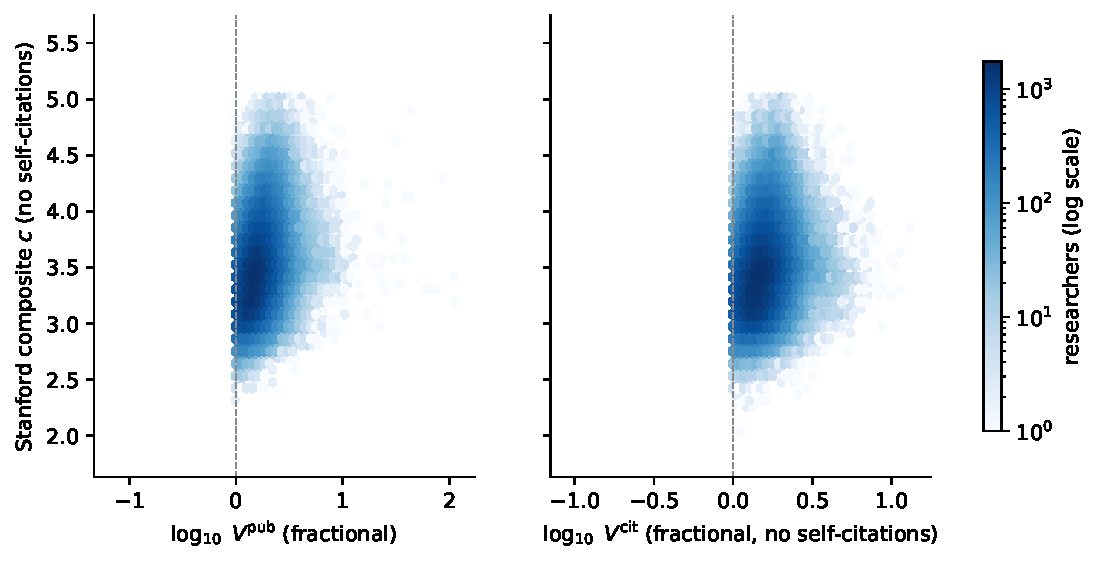
\includegraphics[width=\textwidth]{figures/fig_v_vs_c.pdf}
\caption{Stanford composite indicator $c$ without self-citations against the fractional publication score (left) and the fractional citer score without self-citations (right), for matched researchers in the career table. Shading is the number of researchers on a logarithmic scale.}
\label{fig:v_vs_c}
\end{figure}

\begin{table}[t]
\centering
\caption{Spearman correlations by Stanford field (main field of the researcher) for matched career-table researchers with at least five cited works. The last column compares the citer score with Stanford citations per paper, excluding self-citations. Fields with fewer than 200 matched researchers are omitted.}
\label{tab:fields}
\small
\resizebox{\textwidth}{!}{% generated by researchers/compare_stanford.py
\begin{tabular}{lrrrr}
\toprule
Stanford field & $N$ & $V^{\mathrm{pub}}$ vs $c$ & $V^{\mathrm{cit}}_{\mathrm{ns}}$ vs $c$ (ns) & $V^{\mathrm{cit}}_{\mathrm{ns}}$ vs $n_c/n_p$ (ns) \\
\midrule
Agriculture, Fisheries \& Forestry & 6{,}891 & 0.17 & 0.18 & 0.34 \\
Biology & 8{,}099 & 0.36 & 0.38 & 0.49 \\
Biomedical Research & 16{,}091 & 0.33 & 0.28 & 0.45 \\
Built Environment \& Design & 1{,}227 & 0.25 & 0.23 & 0.09 \\
Chemistry & 12{,}972 & 0.24 & 0.27 & 0.38 \\
Clinical Medicine & 62{,}899 & 0.29 & 0.23 & 0.39 \\
Communication \& Textual Studies & 873 & 0.41 & 0.36 & 0.38 \\
Earth \& Environmental Sciences & 6{,}795 & 0.26 & 0.26 & 0.37 \\
Economics \& Business & 3{,}871 & 0.26 & 0.20 & 0.52 \\
Enabling \& Strategic Technologies & 15{,}873 & 0.25 & 0.22 & 0.43 \\
Engineering & 14{,}649 & 0.29 & 0.29 & 0.38 \\
Historical Studies & 772 & 0.36 & 0.22 & 0.32 \\
Information \& Communication Technologies & 14{,}251 & 0.27 & 0.26 & 0.42 \\
Mathematics \& Statistics & 2{,}266 & 0.18 & 0.27 & 0.50 \\
Philosophy \& Theology & 390 & 0.37 & 0.38 & 0.35 \\
Physics \& Astronomy & 16{,}856 & 0.18 & 0.13 & 0.24 \\
Psychology \& Cognitive Sciences & 3{,}466 & 0.20 & 0.14 & 0.35 \\
Public Health \& Health Services & 3{,}879 & 0.46 & 0.42 & 0.32 \\
Social Sciences & 4{,}627 & 0.29 & 0.29 & 0.42 \\
\bottomrule
\end{tabular}
}
\end{table}

\subsection{Two top-2\% lists}

Drawing up a top-2\% list within each OpenAlex subfield on spectral scores produces a list that overlaps little with Stanford's (Table~\ref{tab:top2}). Only \NTopInStCitfracns{}\% of the \NTopNCitfracns{} researchers in the top 2\% by the fractional citer score without self-citations appear in the Stanford career table, and only \NStInTopCitfracns{}\% of matched Stanford researchers are in that top 2\%. The publication score overlaps more, at \NTopInStPubfrac{}\% and \NStInTopPubfrac{}\% respectively. The difference lies in volume. The median top-2\% researcher by citer score has \NTopMedWorksCit{} eligible works in the corpus and \NTopMedCitesCit{} non-self citations, against \NStMedWorks{} works and \NStMedCites{} citations for the median matched Stanford researcher. A mean rewards a short record of papers cited by influential sources, whereas $c$ rewards a long record of many citations, and the two lists select largely different people.

\begin{table}[t]
\centering
\caption{Top-2\% lists formed within OpenAlex subfields on each spectral score. ``\% on Stanford list'' is the share of the spectral top 2\% matched to a researcher in the Stanford career table, a lower bound because some Stanford researchers are not matched. The last column is the share of matched Stanford researchers who fall in the spectral top 2\%.}
\label{tab:top2}
\small
% generated by researchers/compare_stanford.py
\begin{tabular}{lrrr}
\toprule
Spectral score & Top 2\% (OA subfield) & \% on Stanford list & \% of matched Stanford in top 2\% \\
\midrule
pub, full & 148{,}659 & 7.9 & 6.0 \\
pub, frac & 148{,}659 & 9.2 & 6.9 \\
cit, full & 139{,}623 & 3.4 & 2.4 \\
cit, frac & 139{,}623 & 3.5 & 2.4 \\
cit, full, ns & 134{,}779 & 3.0 & 2.1 \\
cit, frac, ns & 134{,}779 & 3.1 & 2.1 \\
\bottomrule
\end{tabular}

\end{table}

The country composition of the lists also differs (Table~\ref{tab:countries}). The United States accounts for \NShareUsAll{}\% of eligible researchers, \NShareUsSt{}\% of the Stanford career list, \NShareUsCit{}\% of the top 2\% by citer score and \NShareUsPub{}\% of the top 2\% by publication score. China accounts for \NShareCnAll{}\% of eligible researchers but \NShareCnSt{}\% of the Stanford list, \NShareCnCit{}\% of the citer-score list and \NShareCnPub{}\% of the publication-score list. The publication score, which depends on the influence of a researcher's journals and institutions, concentrates the list in the United States more strongly than any citation-based list. Australia accounts for \NShareAuAll{}\% of eligible researchers, \NShareAuSt{}\% of the Stanford list, and \NShareAuCit{}\% and \NShareAuPub{}\% of the two spectral lists. Of the \NAuEligible{} eligible researchers whose last known institution is Australian, \NAuTopCitfracns{} are in the top 2\% of their subfield by citer score and \NAuTopPubfrac{} by publication score, against \NAuStCareer{} Australian entries in the Stanford career table.

\begin{table}[t]
\centering
\caption{Country shares (\%) of the Stanford career list, of the spectral top-2\% lists, and of all eligible OpenAlex researchers, for the twelve countries with the most Stanford-listed researchers. Countries are the researcher's most recent country in each database.}
\label{tab:countries}
\small
% generated by researchers/compare_stanford.py
\begin{tabular}{lrrrr}
\toprule
Country & Stanford career list & $V^{\mathrm{pub}}$ frac & $V^{\mathrm{cit}}$ frac, ns & All eligible \\
\midrule
US & 37.3 & 58.4 & 41.6 & 17.1 \\
GB & 8.8 & 9.0 & 6.8 & 3.6 \\
CN & 6.0 & 5.0 & 8.9 & 18.1 \\
DE & 5.3 & 4.0 & 6.3 & 3.6 \\
CA & 4.1 & 2.2 & 3.2 & 2.3 \\
JP & 3.7 & 0.7 & 3.1 & 4.2 \\
AU & 3.5 & 1.4 & 2.0 & 1.8 \\
FR & 3.1 & 2.0 & 3.9 & 2.8 \\
IT & 3.0 & 0.7 & 1.7 & 2.8 \\
NL & 2.1 & 2.5 & 2.2 & 1.2 \\
ES & 1.7 & 0.8 & 1.6 & 2.5 \\
IN & 1.6 & 0.4 & 0.8 & 4.0 \\
\bottomrule
\end{tabular}

\end{table}

\subsection{Self-citation and counting}

The self-citation shares measured in the two databases agree closely. For matched researchers with at least 50 citations, the Spearman correlation between the OpenAlex self-citation share and Stanford's is \NSelfRho{}, and the medians are \NSelfMedOurs{}\% and \NSelfMedSt{}\%. Across all eligible researchers with at least 50 citations the median is \NSelfMedAll{}\%, and \NSelfOverFortyPct{}\% have more than 40\% self-citations, against \NStSelfOverFortyPct{}\% of the Stanford career list.

Removing self-citations changes the citer score little. The Spearman correlation between the fractional citer scores with and without self-citations is \NRhoCitAllNs{}, and the median researcher moves by \NSelfShiftMed{} percentile points (90th percentile \NSelfShiftNinety{}). For researchers with more than 40\% self-citations, removing them raises the median percentile by \NSelfHiGain{} points rather than lowering it. For these researchers the self-citing papers sit, on average, in sources of lower influence than the papers of their other citers, so removing them raises the mean. A citer score cannot be raised by self-citation unless the self-citing papers appear in sources more influential than those of the researcher's other citers.

The choice between full and fractional counting matters even less. The Spearman correlation between full and fractional scores is \NRhoPubFullFrac{} for the publication score and \NRhoCitFullFrac{} for the citer score. Because both scores are means rather than sums, fractional counting changes only the relative weight of a researcher's own papers, which matters only when their author counts vary widely. The career and single-year citer scores correlate at \NRhoCitCareerSingle{}.

% !TeX root = ../main.tex
% ---------------------------------------------------------------
\section{Discussion}
\label{sec:discussion}
% ---------------------------------------------------------------

The comparison shows that spectral researcher scores and the Stanford composite measure different things. The Stanford list ranks researchers by the accumulated citation record of a career or of a year, and the people at its top have long publication lists and thousands of citations. The spectral scores rank researchers by the typical standing of their papers, judged either by the influence of the journals and institutions that produced them or by the influence of the sources that cite them. Among researchers already on the Stanford list the two are only weakly correlated, and when both are drawn up as top-2\% lists within subfields they select largely different people. The correlation with Stanford's size-independent citations per paper is higher, which locates most of the difference in the treatment of volume rather than in the data sources.

Neither view is the correct one. A cumulative indicator answers the question of whose work has, in total, been most cited, and it is the natural basis for recognising sustained contributions. A mean answers the question of how the typical paper of a researcher is received, and it does not favour long careers or large outputs. Its weakness is the mirror image of the cumulative indicator's. With a threshold of five works, a short record of papers cited from influential sources can place a researcher in the top 2\%, and the median researcher in our citer-score list has only \NTopMedWorksCit{} works. A score of this kind is better read with its supporting counts, and a list that is to be used for recognition would need a higher volume threshold or a ranking that combines the mean with the number of works.

Weighting citations by the influence of their source changes the role of self-citation. Removing self-citations reorders researchers only slightly, and for researchers with heavy self-citation it raises their citer scores rather than lowering them, because their self-citations tend to appear in less influential venues. A mean of citer influence can be raised by citations only if those citations come from sources more influential than the researcher's existing citers, which is precisely what a self-citing researcher or a citation cartel cannot easily arrange. This is the main practical difference from count-based indicators, whose authors must remove self-citations and still caution that citation farms may remain \citep{ioannidisStandardizedCitationMetrics2019a}. The citer score does not detect manipulation, but it gives manipulation little to gain.

The country composition of the lists deserves caution. The publication score inherits the influence of a researcher's journals and institutions, and these are concentrated in the United States and a few other countries, so a ranking on publication score reproduces the hierarchy of institutions as much as it ranks individuals. The citer score is less tied to the researcher's own institution, and its list is closer to the Stanford list in country composition. In both, researchers in China and India are much less represented than among all eligible researchers. This may reflect lower influence of the sources that cite their work, the publication of much of their work in sources that are not retained in the field rankings, or differences in OpenAlex author disambiguation for common names, and our data cannot separate these explanations.

\subsection{Limitations}

Several limitations bear on the comparison, and we note the likely direction of each. First, the matching of Stanford researchers to OpenAlex is by name, location and volume. It recovers four fifths of the career table, and the hand check suggests that most matches are correct, but matching is harder for common names and for early-career researchers, so the matched set probably over-represents senior researchers with distinctive names. Second, OpenAlex author profiles are algorithmic. Split profiles lower a researcher's work count and may remove them from eligibility, and merged profiles mix the papers of different people, which pulls their scores towards the mean. Third, the corpus excludes papers with 30 or more authors and starts in 2000, which removes much of the citation record of researchers in large collaborations and of senior researchers' early work. Fourth, every work is scored by the influence of sources and institutions in 2020--2024, so a paper of 2005 is judged by its journal's present standing rather than its standing at the time. Finally, a citer score rests on the citing works that carry a score, and citations from sources outside the field rankings, probably more common in the humanities and in national-language publishing, are ignored.

\subsection{Conclusion}

We have computed spectral scores for \NOaEligible{} researchers in OpenAlex who meet the Stanford volume baseline, under full and fractional counting, with and without self-citations, for career and single-year citation windows. The scores are open, field-normalised through the influence of sources and institutions, and size-independent. They agree with the Stanford indicators about self-citation, but they rank researchers differently, because they measure the typical reception of a researcher's papers rather than its total. An open alternative to the Stanford list should therefore not be judged by how closely it reproduces that list. The more useful comparison is between what each list rewards. Further work should combine the mean score with volume in a single ranking, test whether the citer score is less affected than $c$ by citation farms identified independently, and repeat the analysis with the sentinel treatment of citations from outside each field.


\bibliographystyle{../spbasic}
\bibliography{../MyLibrary}
\end{document}
